\chapter{Xây dựng real-time platform}

%\section{Rendering of Eyes for Eye-Shape Registrationand Gaze Estimation}

%\section{EyeTab: Model-based gaze estimation on unmodified tablet computers}

\section{...
 \cite{9direction}}
\textbf{Hướng tiếp cận}


% \begin{center}
%     \begin{figure}[h!]
%     \begin{center}
%      \includegraphics[scale=0.5]{}
%     \end{center}
%     \caption{caption}
%     \label{refhinh15}
%     \end{figure}
% \end{center}

%\subsection{Mô hình thuật toán sử dụng}
\textbf{Mô hình thuật toán sử dụng}



\textbf{Kết quả đạt được}
\section{s2 \cite{appearance}}

\textbf{Hướng tiếp cận}

\textbf{Mô hình thuật toán sử dụng}

\newpage
\textbf{Kết quả đạt được}

Bảng bên dưới là  sai số trung bình đạt được với môt số mô hình khác. Bao gồm Random Forests (RF), k-Nearest Neighbours(kNN), Adaptive Linear Regression (ALR), Support Vector Regression (SVR).
\begin{center}
    \begin{figure}[h!]
    \begin{center}
     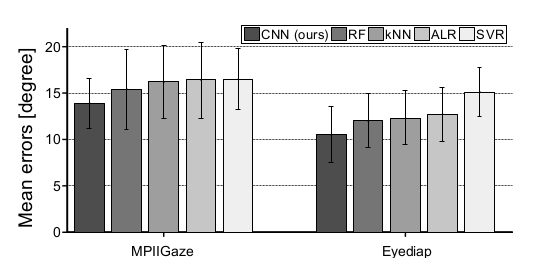
\includegraphics[scale=0.5]{img/2dataset.png}
    \end{center}
    \caption{Bảng thống kê kết quả}
    \label{refhinh20}
    \end{figure}
\end{center}
\section{Rendering of Eyes for Eye-Shape Registration and Gaze Estimation
\cite{eyeShapeRegistrationAndGazeEstimation}}
Nhóm nghiên cứu tạo ra một số lượng lớn hình ảnh thực tế của mắt bằng cách sử dụng mô hình vùng mắt động. Chúng được sử dụng làm dữ liệu đào tạo để đăng ký hình dạng mắt và ước tính dựa trên sự xuất hiện dựa trên sự xuất hiện.
\begin{center}
    \begin{figure}[h!]
    \begin{center}
     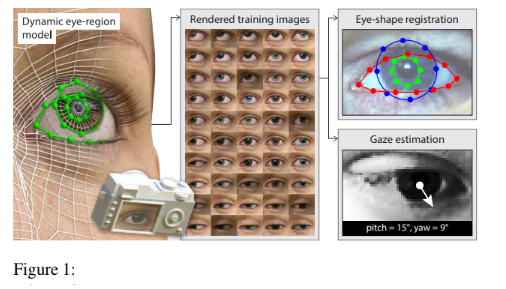
\includegraphics[scale=1]{img/photorealistic_images_of_eyes.png}
    \end{center}
    \caption{Chúng tôi tạo ra một số lượng lớn các hình ảnh photorealistic của mắt bằng cách sử dụng một mô hình vùng mắt động.}
    \label{refhinh20}
    \end{figure}
\end{center}
\textbf{Hướng tiếp cận}

(a) Quét hình ảnh 3D dày đặc (1,4 triệu đa giác (polygons))

(b) Được tái hiện lại thành dạng tối ưu cho hoạt ảnh (9,005 đa giác (polygons))

(c) Các chi tiết bề mặt da có độ phân giải cao được khôi phục bằng bản đồ dịch chuyển 

(d) Các điểm mốc mí mắt và mí mắt 3D được chú giải bằng tay 

(e) Hiển thị mẫu được hiển thị 
\begin{center}
    \begin{figure}[h!]
    \begin{center}
     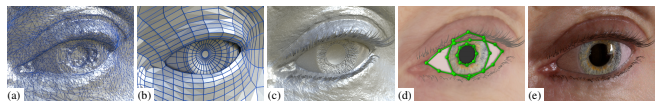
\includegraphics[scale=0.75]{img/An_overview_of_our_model_preparation_process.png}
    \end{center}
    \caption{Tổng quan về quá trình chuẩn bị mô hình.}
    \label{refhinh20}
    \end{figure}
\end{center}
Mô hình mắt nghiên cứu bao gồm các sclera, học sinh, mống mắt, và giác mạc (a) (the sclera, pupil, iris, and cornea) và có thể thể hiện sự thay đổi thực tế trong cả hai hình dạng (giãn nở đồng tử) và kết cấu (màu iris, tĩnh mạch scleral) (b).
\begin{center}
    \begin{figure}[h!]
    \begin{center}
     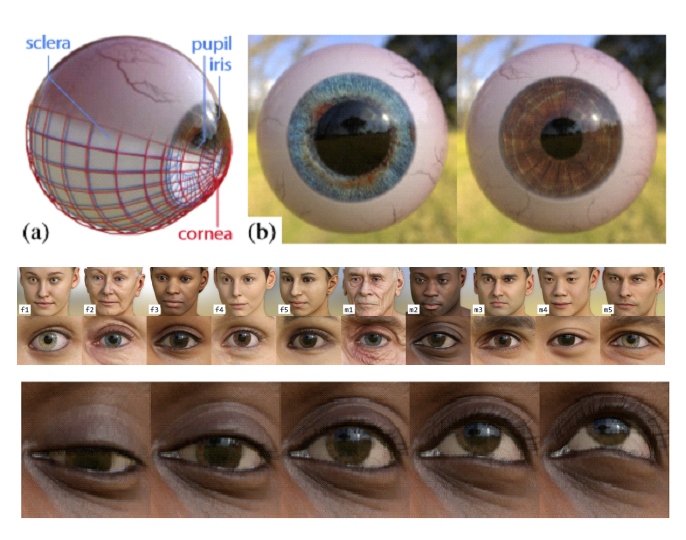
\includegraphics[scale=0.75]{img/Eye_model_and_3D_head_model.png}
    \end{center}
    \caption{Mô hình mắt và mô hình đầu (3D).}
    \label{refhinh20}
    \end{figure}
\end{center}

Máy ảnh được định vị để mô phỏng các thay đổi trong tư thế đầu (a). Tại vị trí này, chúng tôi hiển thị nhiều hình ảnh mắt cho các hướng nhìn khác nhau bằng cách đặt mô hình nhãn cầu (b):
\begin{center}
    \begin{figure}[h!]
    \begin{center}
     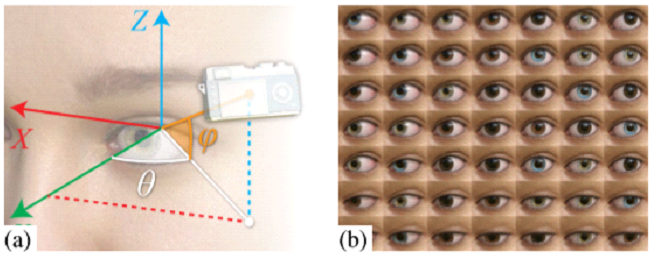
\includegraphics[scale=0.75]{img/Camera_position.png}
    \end{center}
    \caption{Vị trí máy ảnh.}
    \label{refhinh20}
    \end{figure}
\end{center}

Bốn bản đồ môi trường HDR, sử dụng cho ánh sáng thực tế: sáng / ngoài trời nhiều mây và sáng / tối trong nhà. Màu đỏ thể hiện điểm số tồi tệ nhất.

\begin{center}
    \begin{figure}[h!]
    \begin{center}
     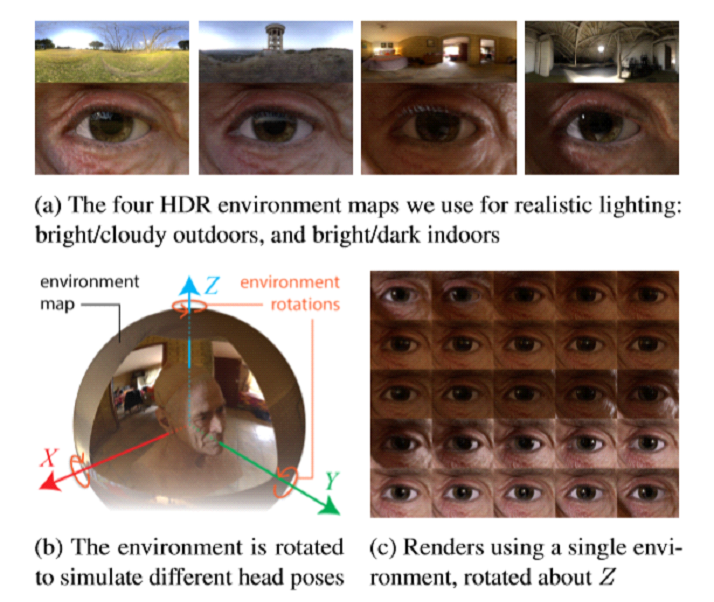
\includegraphics[scale=0.5]{img/Appearance_variation_from_lighting.png}
    \end{center}
    \caption{Sự biến đổi từ việc thay đổi ánh sáng được mô hình hóa với ảnh chụp có môi trường có phạm vi năng động cao.}
    \label{refhinh20}
    \end{figure}
\end{center}

\begin{center}
    \begin{figure}[h!]
    \begin{center}
     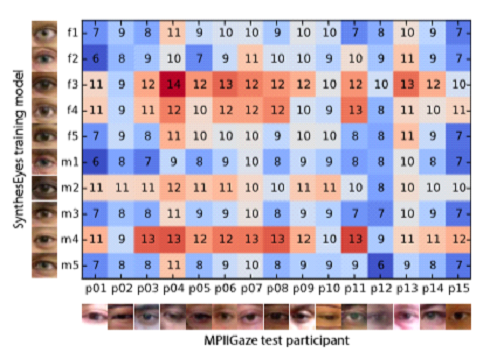
\includegraphics[scale=0.5]{img/Estimation_of_errors_on_MPIIGaze.png}
    \end{center}
    \caption{Ước lượng lỗi trên MPIIGaze}
    \label{refhinh20}
    \end{figure}
\end{center}
Nhóm nghiên cứu đã trình bày một phương pháp mới để tổng hợp những hình ảnh cận cảnh thực tế được dán nhãn hoàn hảo của mắt người. Một đường ống đồ họa máy tính sử dụng một bộ sưu tập các mô hình vùng mắt động thu được từ quét đầu để tạo ra các hình ảnh cho thấy phạm vi của các tư thế đầu, hướng nhìn và điều kiện chiếu sáng. Nhóm nghiên cứu đã chứng minh rằng phương pháp nghiên cứu hoạt động tốt hơn các phương pháp hiện đại để đăng ký hình dạng mắt và ước tính dựa trên sự xuất hiện dựa trên dữ liệu chéo trong tự nhiên. Những kết quả này hứa hẹn và nhấn mạnh tiềm năng quan trọng của các phương pháp tổng hợp học tập như vậy, đặc biệt là sự bứt phá với các phương pháp giám sát quy mô lớn gần đây.
\textbf{Kết quả đạt được}
Ví dụ về độ phù hợp (fits) với SynthesEyes eye-CLNF về hình ảnh trong tự nhiên (a) và hình ảnh webcam (b). Hai hàng hình ảnh trên cùng minh họa cho việc nhận dạng hình dạng mắt thành công, trong khi hàng dưới cùng minh họa các trường hợp thất bại, bao gồm các vệt chưa được tạo ra (tóc), các tư thế chưa được chỉnh sửa (mắt kín), kính và khởi tạo mô hình không chính xác.
\begin{center}
    \begin{figure}[h!]
    \begin{center}
     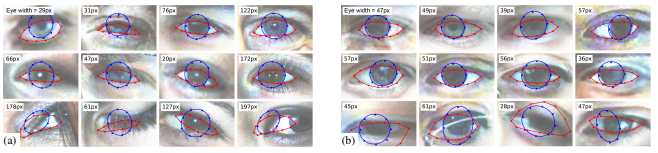
\includegraphics[scale=0.75]{img/Example_fits_of_our_SynthesEyes_eye_CLNF.png}
    \end{center}
    \caption{Ví dụ về độ phù hợp (fits) với SynthesEyes eye-CLNF}
    \label{refhinh20}
    \end{figure}
\end{center}
Trục x đại diện cho tập huấn luyện được sử dụng. Dấu chấm là các lỗi trung bình và đường màu đỏ thể hiện một giới hạn thấp hơn về mặt xác thực (số điểm xác thực chéo trong tập dữ liệu).

\begin{center}
    \begin{figure}[h!]
    \begin{center}
     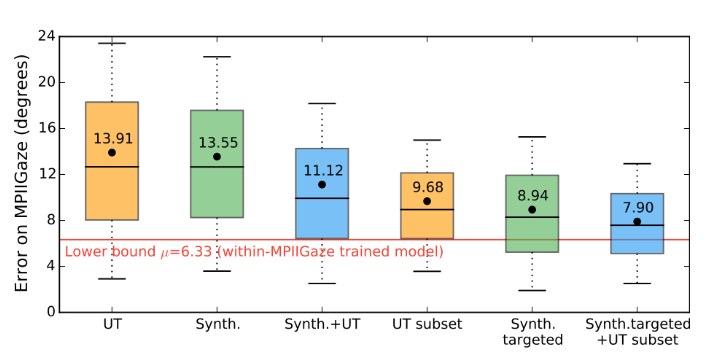
\includegraphics[scale=0.70]{img/Performance_chart_on_MPIIGaze.png}
    \end{center}
    \caption{Biểu đồ hiệu suất trên MPIIGaze}
    \label{refhinh15}
    \end{figure}
\end{center}

\section{Learning an appearance-based gaze estimator from one million synthesised images \cite{Learninganappearancebasedgazeestimator}}

\textbf{Hướng tiếp cận}

Nghiên cứu đã cung cấp một triệu hình ảnh thực tế về mắt bằng cách sử dụng mô hình vùng mắt được mô phỏng. Chúng được kết hợp với một hình ảnh đầu vào bằng cách sử dụng một phương pháp tiếp cận hàng xóm gần nhất (nearest-neighbor approach) để ước lượng cái nhìn. Mô hình quản lý này tìm ra các kết quả phù hợp ngay cả với các góc nhìn cực độ và ánh sáng chói từ kính.

\begin{center}
    \begin{figure}[h!]
    \begin{center}
     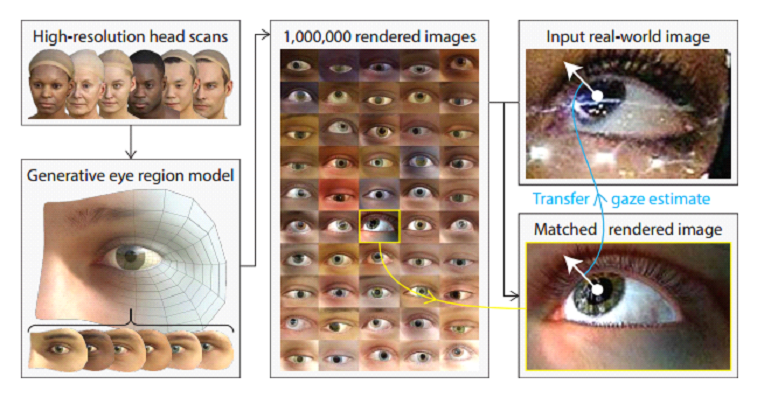
\includegraphics[scale=0.70]{img/Image_dataset_the_nearest_neighbor_approach.png}
    \end{center}
    \caption{Sử dụng phương pháp tiếp cận hàng xóm gần nhất(nearest-neighbor approach) để ước lượng cái nhìn.}
    \label{refhinh15}
    \end{figure}
\end{center}

Nhóm nghiên cứu trình bày về UnityEyes, một phương pháp mới để tổng hợp nhanh chóng số lượng lớn các hình ảnh vùng mắt thay đổi cho dữ liệu huấn luyện. Phương pháp nghiên cứu này: kết hợp một mô hình 3D sinh học mới lạ của vùng mắt người với khung thời gian thực. Mô hình vùng mắt có nguồn gốc từ quét khuôn mặt 3D có độ phân giải cao và sử dụng xấp xỉ thời gian thực cho các vật liệu và cấu trúc nhãn cầu phức tạp, cũng như các phương pháp hình học thủ tục lấy cảm hứng từ giải phẫu cho hoạt ảnh mí mắt. Tổng hợp hình ảnh bằng cách sử dụng trình kết xuất đồ họa và ánh sáng dựa trên hình ảnh thực tế và đa dạng điều kiện chiếu sáng. Những hình ảnh tổng hợp này có thể được khớp với hình ảnh đầu vào trong thế giới thực bằng cách sử dụng các phương pháp tiếp cận gần nhất để ước lượng ánh mắt. 

\begin{center}
    \begin{figure}[h!]
    \begin{center}
     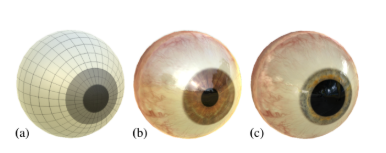
\includegraphics[scale=1]{img/Eyeball_mesh.png}
    \end{center}
    \caption{Hình ảnh về lưới mắt: (a) được hiển thị với các vật liệu dựa trên vật lý và các hiệu ứng khúc xạ, mô hình co rút đồng tử (b) và giãn nở (c).}
    \label{refhinh15}
    \end{figure}
\end{center}

\begin{center}
    \begin{figure}[h!]
    \begin{center}
     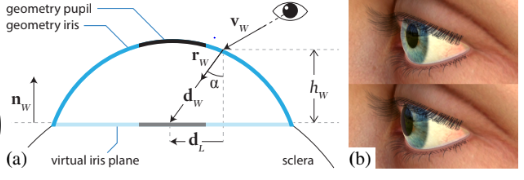
\includegraphics[scale=1]{img/Model_iris_refraction.png}
    \end{center}
    \caption{Mô hình khúc xạ iris bằng cách thay đổi kết cấu tra cứu: Một điểm ảnh được xem khúc xạ chính xác để hiển thị màu đen (tròng mắt) thay vì màu xanh (bề mặt hình học).}
    \label{refhinh15}
    \end{figure}
\end{center}

\begin{center}
    \begin{figure}[h!]
    \begin{center}
     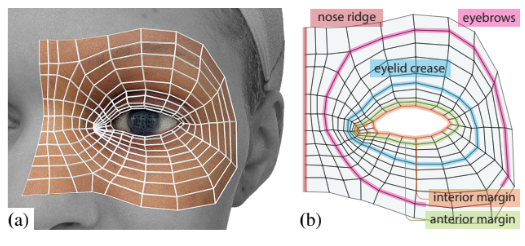
\includegraphics[scale=1]{img/Generative_eye_region_model.PNG}
    \end{center}
    \caption{Mô hình khởi tạo vùng mắt: (a) Cho thấy cấu trúc liên kết vùng mắt chung của chúng ta (229 đỉnh) trên một quét thô (khoảng 5M đỉnh). (b) Cho thấy cấu trúc liên kết trong không gian kết cấu uv với các vòng cạnh quan trọng được đánh dấu.}
    \label{refhinh15}
    \end{figure}
\end{center}

\textbf{Kết quả đạt được}

Nearest-neighbour pairs hiển thị hình ảnh tự nhiên (trên cùng) và phần kết của chúng tôi (dưới cùng) cùng với ánh mắt được ước tính (màu xanh lá cây).
Ba hàng đầu hiển thị ước tính chất lượng tốt, ngay cả dưới ánh sáng khó khăn (thiếu ánh sáng), độ phân giải thấp và góc nhìn cực đoan.
Hàng dưới cùng hiển thị các trường hợp lỗi từ biến thể chưa được sửa đổi, ví dụ: trang điểm và tóc.

\begin{center}
    \begin{figure}[h!]
    \begin{center}
     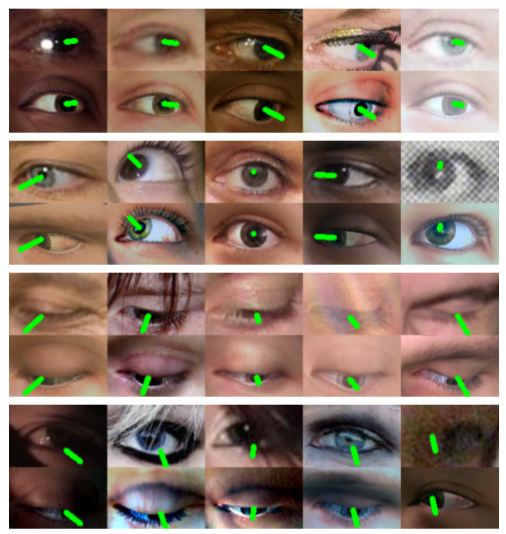
\includegraphics[scale=0.7]{img/The_result_of_Nearest_neighbour_pairs.png}
    \end{center}
    \caption{Kết quả của phương pháp tổng hợp những hình ảnh cận cảnh thực tế (Nearest-neighbour pairs) được dán nhãn hoàn hảo của mắt người }
    \label{refhinh15}
    \end{figure}
\end{center}

Lỗi pixel và điểm nhìn của phương pháp nearest-neighbor tương ứng với tập UnityEyes và MPIIGaze. Nhóm nguyên cứu đạt được lỗi thấp nhất ở 1.4 triệu hình ảnh.


\begin{center}
    \begin{figure}[h!]
    \begin{center}
     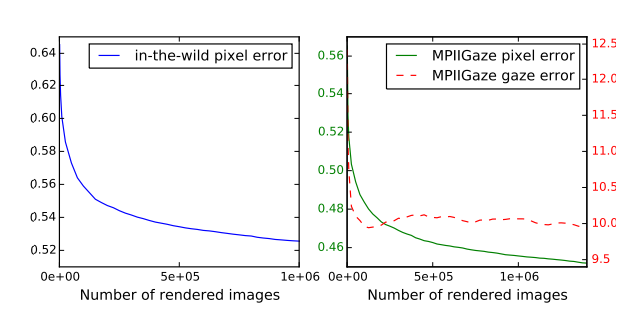
\includegraphics[scale=1]{img/Pixel_and_gaze_errors_for_nearest_neighbor.png}
    \end{center}
    \caption{Lỗi pixel và điểm nhìn của phương pháp nearest-neighbor tương ứng với tập UnityEyes và MPIIGaze. Nhóm nguyên cứu đạt được lỗi thấp nhất ở 1.4 triệu hình ảnh.}
    \label{refhinh15}
    \end{figure}
\end{center}


\newpage



